%%%%%%%%%%%%%%%%%%%%  練習問題（旧 prob_p35.png / prob_p36.png）  %%%%%%%%%%%%%%%%%%%%
% 第2章（熱力学）から問題番号を［1］に振り直す（原本もここで番号がリセットされている）
\setcounter{qno}{0}

\Rank{A問題}

\Mon{基本事項の確認}

\hspace{1zw}以下の設問に答えよ．ただし，気体定数は$8.31\U{J/mol\cdot K}$である．
\begin{komon}
\ko{1} シリンダー内に断面積$1.0\times 10^{-2}\U{m^2}$のピストンで閉じ込められた気体が，$5.0\U{N}$の力でピストンを押している．この気体の圧力は何$\U{Pa}$か．有効数字2桁で求めよ．
\ko{2} 酸素気体$\mathrm{O_2}$ $96\U{g}$中に含まれている酸素分子の数は何個か．ただし，アボガドロ数を$N_{\mathrm{A}}=6.02\times 10^{23}$\,[個/mol]とする．有効数字2桁で求めよ．
\ko{3} 温度$20\U{C}$の水$300\U{g}$を$100\U{C}$まで加熱するのに必要な熱量は何$\U{cal}$か．またこれは何$\U{J}$か．ただし，熱の仕事当量を$J=4.2\U{J/cal}$とする．有効数字2桁で求めよ．
\ko{4} 質量$200\U{g}$の金属塊の温度を$20\U{C}$から$60\U{C}$まで加熱するのに要する熱量が$56000\U{cal}$であった．この金属の比熱は何$\U{cal/g\cdot K}$か．また，この金属塊の熱容量は何$\U{cal/K}$か．有効数字2桁で求めよ．
\end{komon}

\Rank{B問題}

\Mon{状態方程式}

\hspace{1zw}容器中に理想気体が入っており，圧力$p_0\U{Pa}$，体積$V_0\U{m^3}$におけるその気体の温度を$T_0\U{K}$とする．
\begin{komon}
\ko{1} 温度を$T_0\U{K}$に保ったまま，体積を$kV_0\U{m^3}$になるまで膨張したときの気体の圧力を求めよ．
\ko{2} 圧力を$p_0\U{Pa}$に保ったまま，温度が$kT_0\U{K}$になるまで加熱したときの気体の体積を求めよ．
\ko{3} 体積を$V_0\U{m^3}$に保ったまま，圧力が$kp_0\U{Pa}$になるまで熱したときの気体の温度を求めよ．
\ko{4} この気体を熱し続けて温度が$t_1\U{C}$になったとき，圧力が$p_1\U{Pa}$であったとする．$0\U{C}=273.15\U{K}$として，気体の体積を求めよ．
\end{komon}

\Mon{状態方程式}\Sitei

\begin{zuright}{47mm}
\hspace{1zw}右図のように断熱材でできた自由に動くことのできるピストン$\mathrm{C}$で，長さ$l_{\mathrm{A}}\U{m}$の$\mathrm{A}$と長さ$l_{\mathrm{B}}\U{m}$の$\mathrm{B}$の二つの部分に分けられた容器があり，$\mathrm{A}$，$\mathrm{B}$にはともに温度$T_0\U{K}$，圧力$p_0\U{Pa}$の理想気体が入っている．$\mathrm{A}$内の気体はそのままにし，$\mathrm{B}$内の気体だけを温めて温度を$T_1\U{K}$に上げて保ったところ，$\mathrm{C}$は$l\U{m}$だけ移動した．
\begin{komon}
\ko{1} $\mathrm{C}$はどちら向きへ移動するか．
\ko{2} 移動後の$\mathrm{A}$内の気体の温度および，$\mathrm{A}$，$\mathrm{B}$内の気体の圧力を求めよ．
\end{komon}
\zusep
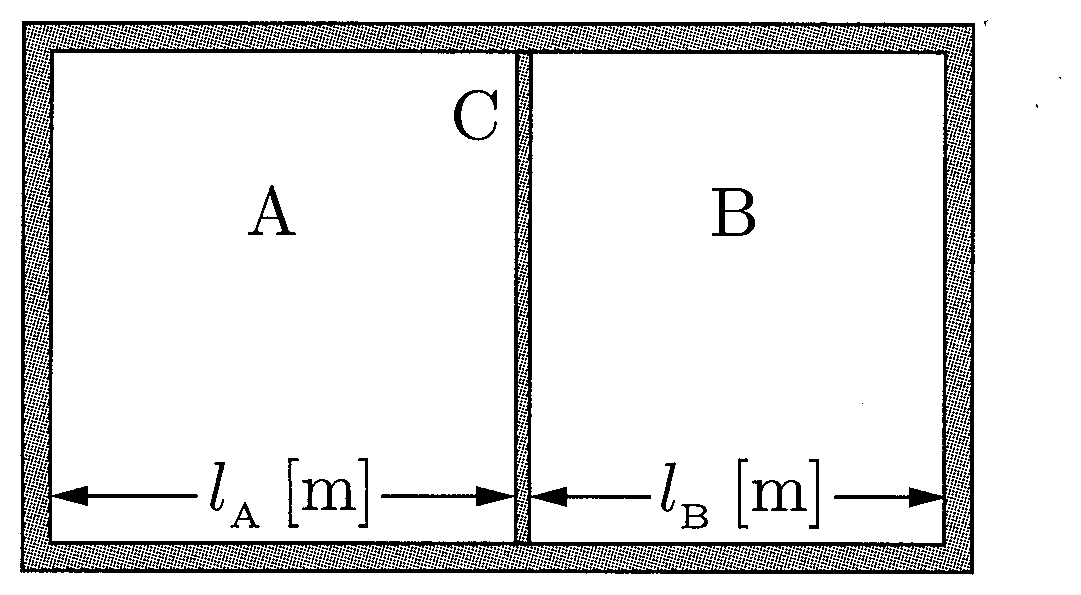
\includegraphics[keepaspectratio,width=47mm]{fig/ch14_p35_cyl.png}
\end{zuright}

\Mon{熱量の保存}\Sitei

\hspace{1zw}比熱$c_{\mathrm{A}}\U{cal/g\cdot K}$，質量$m_{\mathrm{A}}\U{g}$，温度$t_{\mathrm{A}}\U{C}$の金属$\mathrm{A}$と，比熱$c_{\mathrm{B}}\U{cal/g\cdot K}$，質量$m_{\mathrm{B}}\U{g}$，温度$t_{\mathrm{B}}\U{C}$の金属$\mathrm{B}$を接触させ十分時間が経ったところ，$\mathrm{A}$，$\mathrm{B}$間で熱のやり取りが行われ，熱平衡状態に達した．$t_{\mathrm{A}}>t_{\mathrm{B}}$として以下の問に答えよ．
\begin{komon}
\ko{1} 熱平衡状態における$\mathrm{A}$，$\mathrm{B}$の温度を求めよ．
\ko{2} このとき$\mathrm{A}$の失った熱量および$\mathrm{B}$が得た熱量を求めよ．
\end{komon}

\Mon{熱量の保存}

\hspace{1zw}質量$M\U{g}$の銅製の容器（温度$t_0\U{C}$）に温度$t_0\U{C}$の水が$w\U{g}$入っている．この中へ温度$t\U{C}$（$t>t_0$），質量$m\U{g}$の銅球を入れてかきまぜたところ，全体の温度は一様に$t'\U{C}$になった．これらを元に，銅の比熱を求めよ．
% 誤植訂正（2026-08-29）：元の問題集は「この中への温度 t[C]（t>t_0），質量 m[g] の銅球を
%   入れて」となっていたが，「この中へ温度 t[C]…の銅球を入れて」が正しい（「への」の「の」が余分）．

\Mon{摩擦熱}

\hspace{1zw}時速$72\U{km/h}$で走っている質量$1\U{t}$の自動車がブレーキをかけたところ，自動車は摩擦のため静止した．摩擦によって生じた熱量は何$\U{cal}$か．ただし熱の仕事当量を$J=4.2\U{J/cal}$とする．

\Mon{熱力学第一法則}

\hspace{1zw}ある気体が状態変化する際，気体に外界から加えられた熱量，気体の内部エネルギーの増加量，そして気体が外界に対してした仕事がそれぞれ$Q\U{J}$，$\Delta U\U{J}$，$W\U{J}$であった．これについて以下の問に答えよ．
\begin{komon}
\ko{1} $Q$, $\Delta U$, $W$の間に成り立つ熱力学第一法則を記せ．
\end{komon}
\hspace{1zw}またこの状態変化の際の仕事・熱のやり取りを，気体が熱を外界に放出し，気体が外界から仕事をされたとして捉え，それぞれの量を$Q'\U{J}$，$W'\U{J}$とおく．
\begin{komon}
\ko{2} $Q'$, $\Delta U$, $W'$の間に成り立つ関係式を求めよ．
\end{komon}

\Rank{C問題}

\Mon{状態方程式}

\begin{zuright}{41mm}
\hspace{1zw}図のように容積の等しい二つの容器$\mathrm{A}$，$\mathrm{B}$が細管でつながれ，コック$\mathrm{C}$を通して温度$T_1\U{K}$，圧力$P_1\U{Pa}$の大気に通じている．はじめコック$\mathrm{C}$は開かれており，容器および内部の気体の温度はすべて大気と同じ温度であった．細管の容積と容器の熱膨張を無視し，空気は理想気体とみなしてよいものとして以下の問に答えよ．
\zusep
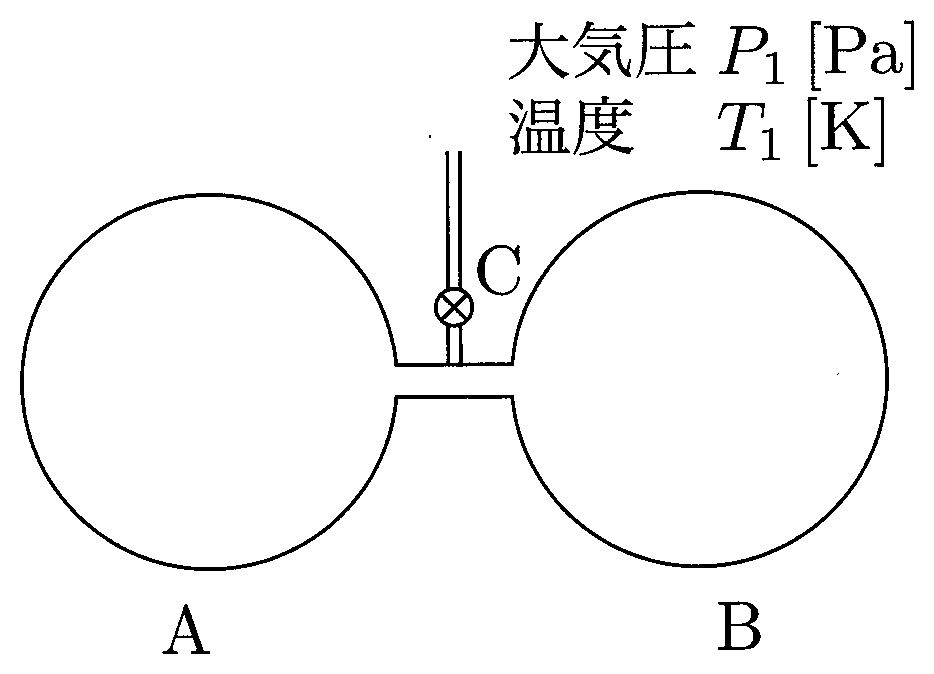
\includegraphics[keepaspectratio,width=41mm]{fig/ch14_p36_flask.png}
\end{zuright}
\vspace{-\medskipamount}
\begin{komon}
\ko{1} コック$\mathrm{C}$を開いたまま，$\mathrm{B}$は大気と同じ温度に保ちつつ$\mathrm{A}$の温度を$T_0\U{K}$になるまでゆっくりと冷やした．$\mathrm{A}$を冷やしている間に$\mathrm{A}$，$\mathrm{B}$に流入した気体のモル数は，はじめ$\mathrm{B}$の中にあった空気のモル数の何倍か．
\ko{2} 次にコック$\mathrm{C}$を閉じ，$\mathrm{A}$をゆっくりと温めて，$\mathrm{A}$および$\mathrm{B}$の温度を再び大気の温度に等しくした．このときの$\mathrm{A}$，$\mathrm{B}$内の空気の圧力$P_2\U{Pa}$を求めよ．
\end{komon}

\Mon{熱力学第二法則}

\hspace{1zw}次の文の空欄に当てはまる語を下記の語群の中から選び，その記号で答えよ．ただし，重複して用いてもよいものとする．

\hspace{1zw}熱力学第二法則は，\framebox[3zw]{ア}変化に関係した法則で，さまざまな表現の仕方がある．
\begin{quote}
\noindent $\mathrm{I}$\hspace{2zw}クラウジウスの原理\par
\hspace{2zw}他に影響を与えないで，熱を\framebox[3zw]{イ}温の物体から\framebox[3zw]{ウ}温の物体に移すことはできない．\par
\noindent $\mathrm{I\!I}$\hspace{2zw}トムソンの原理\par
\hspace{2zw}与えられた\framebox[3zw]{エ}をすべて\framebox[3zw]{オ}に変えてしまうような熱機関をつくることはできない．
\end{quote}
\hspace{1zw}$\mathrm{I}$と$\mathrm{I\!I}$は，同じ内容を違う表現で述べてあるにすぎない．同値であることは，数学でよく用いられる対偶法によって証明することができる．これを考えてみよう．

\hspace{1zw}もし，$\mathrm{I\!I}$が成り立たないとすると，\framebox[3zw]{カ}温の熱源からもらった熱をすべて\framebox[3zw]{キ}に変えることができるから，これを\framebox[3zw]{ク}温の熱源に与えれば\framebox[3zw]{ケ}を与えたのと同じことになるので，他に影響を与えないで熱が\framebox[3zw]{コ}温の物体から\framebox[3zw]{サ}温の物体に移ったことになり，$\mathrm{I}$が否定されてしまう．同様に$\mathrm{I}$が成り立たないとすると，$\mathrm{I\!I}$が否定されるので，$\mathrm{I}$と$\mathrm{I\!I}$とは同値の関係にあると言える．

\begin{itembox}[l]{【選択肢】}
\noindent\hspace*{1zw}A\hspace{1zw}熱\hfill B\hspace{1zw}仕事\hfill C\hspace{1zw}高\hfill D\hspace{1zw}低\hfill E\hspace{1zw}可逆\hfill F\hspace{1zw}不可逆\hspace*{1zw}
\end{itembox}
